\documentclass{article}
\usepackage{amsfonts, amsmath, amssymb, amsthm, dsfont, mathtools, stmaryrd}
\usepackage{enumitem}
\usepackage{graphicx}
\usepackage{setspace}
\usepackage{indentfirst}
\usepackage[margin=1in]{geometry}
\graphicspath{{./images/}}
\setstretch{1.15}
\newtheorem{theorem}{Theorem}
\newtheorem{definition}{Definition}
\newtheorem{lemma}{Lemma}
\newcommand*{\R}{\mathbb{R}} 
\newcommand*{\N}{\mathbb{N}}
\newcommand*{\Z}{\mathbb{Z}}
\newcommand*{\M}{\mathcal{M}}

\title{M54 conjecture}
\author{Neo Lee}
\date{November 2023}

% https://www.math.ucla.edu/~pak/papers/how-to-write1.pdf
% https://web.mit.edu/jrickert/www/mathadvice.html
% https://terrytao.wordpress.com/advice-on-writing-papers/ https://arxiv.org/abs/2209.07451

\begin{document}

\maketitle

\section{\centering Abstract}
This paper proves a conjecture related to the necessary and sufficient condition for the
time-invariant Nash equilibrium for the stake-governed random turn game -- Trail of Lost Pennies --
introduced by [Hammond]. Trail of Lost Pennies is a variant of tug-of-war, a class of games that has
a history dates back to [some year] by [author name]. 

\section{\centering Introduction}
The Trail of Lost Pennies is a two-player strategic game played on the integer line introduced by
[Hammond]. Below, we will first introduce the finite Trail of Lost Pennies, then its infinite
counterpart. In the end of this section, we will bridge the gap between the two versions of the game
and use the finite version to motivate our results in infinite Trail of Lost Pennies. (Note: Trail
of Lost Pennies refers to the infinite version unless otherwise specified.)

\subsection{\centering Finite Trail of Lost Pennies}
\begin{figure}[htb!]
    \centering
    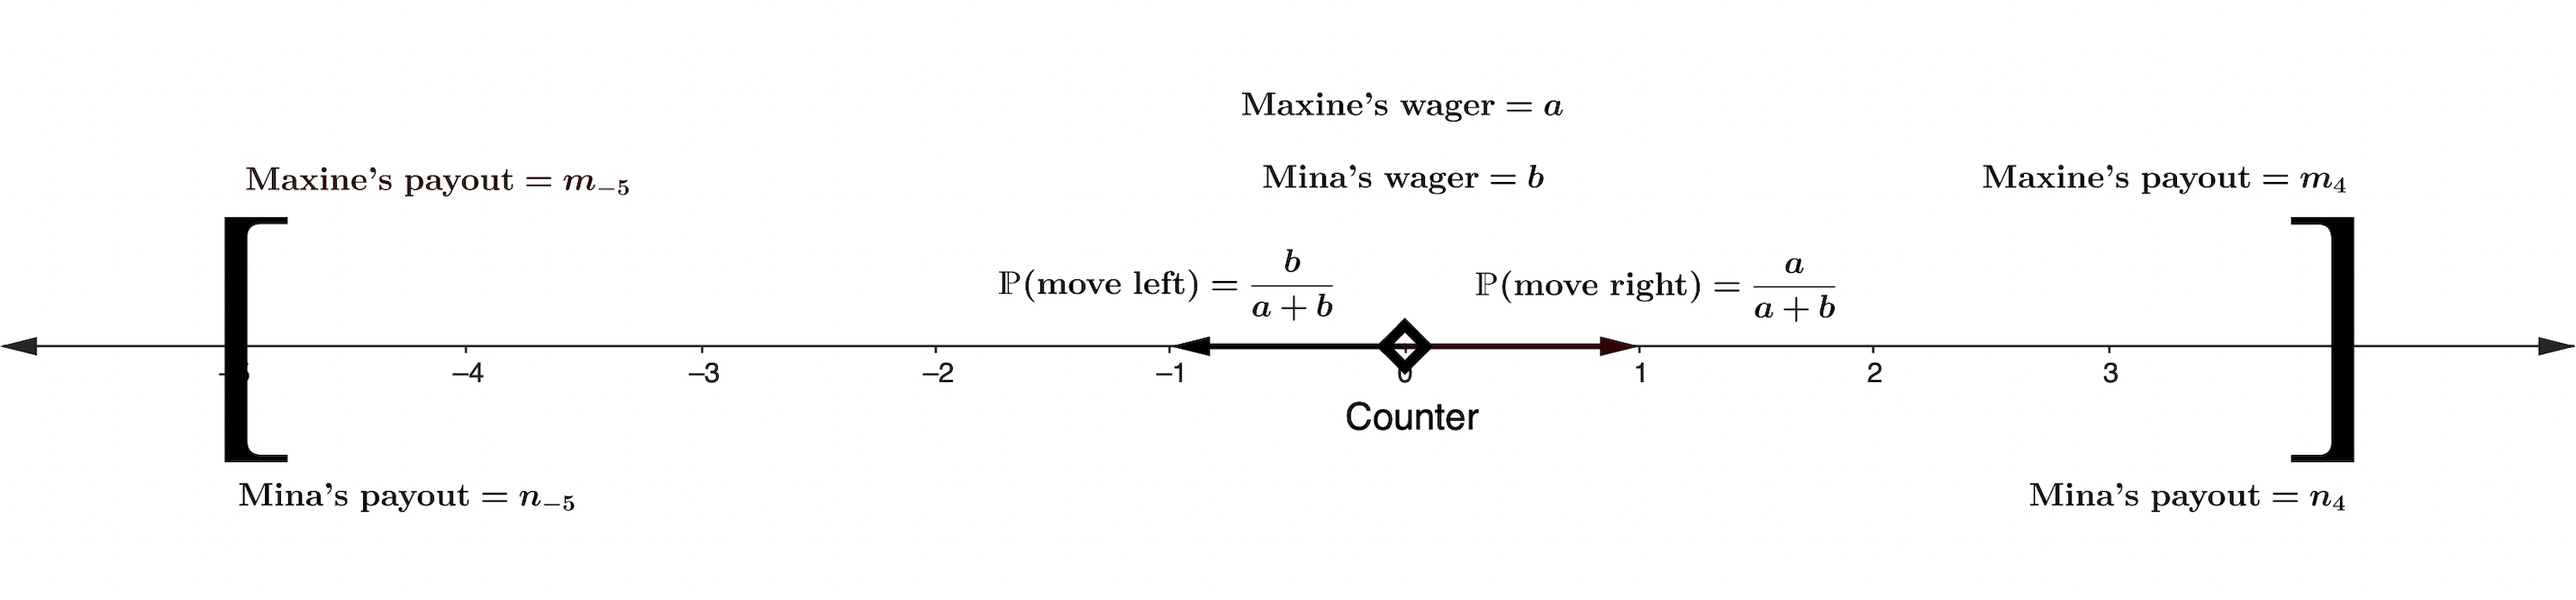
\includegraphics[scale=0.3]{finite_trail.png}
    \caption{Trail($m_{-5}, m_{4}, n_{-5}, n_{4}$) on $\llbracket-5, 4\rrbracket$}
\end{figure}

The game is best illustrated by an example. Here we consider the finite Trail game playing on the
finite integer interval $\llbracket-5, 4\rrbracket$. We also introduce two players Maxine (who plays
to the right) and Mina (who plays to the left), who are infinitely wealthy. The game starts with a
counter placed at the origin. At each turn, Maxine and Mina wager $a$ and $b$ amount respectively.
The counter then moves one step to the left or right with probability proportional to the wager of
the player on that side, specifically $$\mathds{P}(\text{move left}) = \frac{b}{a+b} \quad
\text{and} \quad \mathds{P}(\text{move right}) = \frac{a}{a+b}.$$ The games repeats until the
counter reaches either end of the line, namely $-5$ or $4$. If the counter reaches $-5$, Maxine will
receive $m_{-5}$ amount and Mina will receive $n_{-5}$ amount minus their total wager throughout the
game. If the counter reaches $4$, Maxine will receive $m_{4}$ amount and Mina will receive $n_{4}$
amount minus their total wager throughout the game.

Notice that $m_{-5}, m_4, n_{-5}, n_4$ are predefined values to set up the game such that
$m_{-5}<m_4$ and $n_4<n_{-5}$, which tells us that Maxine is always playing to the right to maximize
her payout and Mina is always playing to the left. 

\subsection{\centering Infinite Trail of Lost Pennies}
\begin{figure}[htb!]
    \centering
    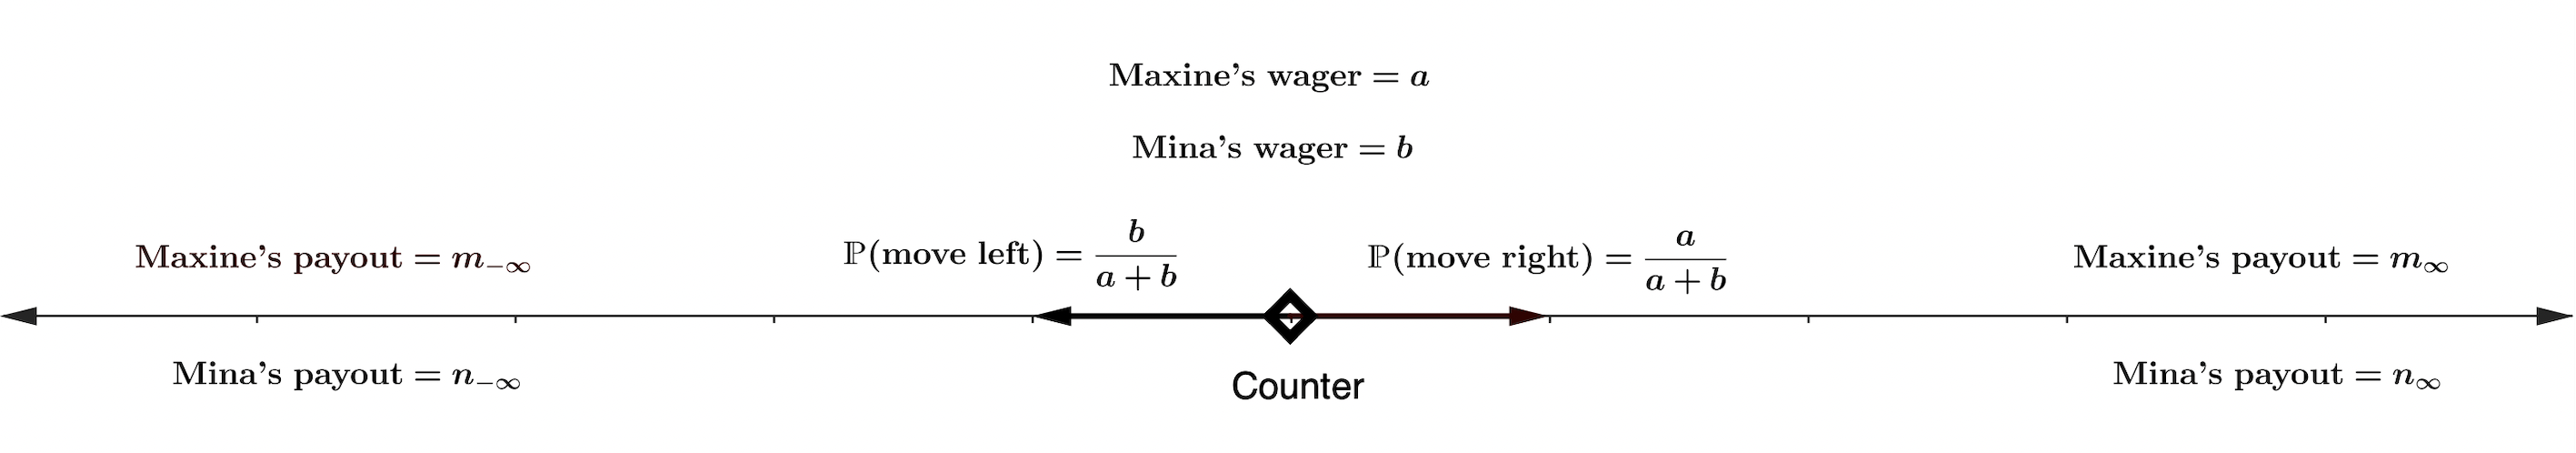
\includegraphics[scale=0.3]{infinite_trail.png}
    \caption{Trail($m_{-\infty}, m_{\infty}, n_{-\infty}, n_{\infty}$)}
\end{figure}

The infinite Trail game is very similar to the finite version, except that the game is played on the 
infinite integer line $\Z$ and the counter can move infinitely far to the left or right. The game


A traditional constant-biased tug-of-war involves tossing a biased coin to determine whether a
counter moves left or right at each turn. The game ends when the counter reaches either end of the
line. If the counter reaches the left end, the left player wins; if the counter reaches the right
end, the right player wins. Put it in mathematical terms, the game is essentially a one-dimensional
random walk.

Now consider a variant of the constant-biased tug-of-war, where the coin bias changes according to
the player's wager. In this game, the left player, Maxine, and the right player, Mina, each assumed
to be infinitely wealthy, will wager $a$ and $b$ amount respectively at each turn. The coin bias is
then determined by the ratio of the wagers, i.e. the probability of the counter moving left is
$\frac{a}{a+b}$ and the probability of the counter moving right is $\frac{b}{a+b}$. The game ends
when the counter reaches either end of the line. If the counter reaches the left end, Maxine wins;
if the counter reaches the right end, Mina wins. Therefore, the game is no longer an ordinary
one-dimensional random walk, but a random walk with varying probability depending on both players'
strategy at each turn. This variant of tug-of-war is termed player-funded stake-governed tug-of-war.

Unlike traditional tug-of-war, which is a
test of strength, this game challenges the intellect, requiring players to navigate a landscape of
chance and choice. Introduced by Hammond, the game serves as a rich platform for exploring complex
mathematical ideas in a seemingly simple setup.

At its core, 'Trail of Lost Pennies' is played on an infinite sequence of integers, representing
positions on a line. Two players, each with their own objectives, compete to move a counter along
this line. The game is not just about moving back and forth; it encapsulates a deeper understanding
of strategy under uncertainty. Each decision made by the players isn't just about the immediate move
but also about influencing the future course of the game.

The significance of studying 'Trail of Lost Pennies' lies in its ability to model real-world
scenarios where decisions are made under uncertainty. It provides a simplified yet profound way to
understand how choices can be strategically made when outcomes are influenced by chance. This paper
aims to demystify the complexities of the game and make its concepts accessible, particularly
focusing on the time-invariant Nash equilibrium, which stands as a pivotal concept in understanding
the game's strategic depth.

In the following sections, we will take a step-by-step approach to unfold the game's intricacies,
starting from a simplified version for ease of understanding and gradually moving towards its
comprehensive mathematical model. This approach is designed to make the paper engaging and
informative for both those new to the game and those well-versed in its mathematical foundation.



\subsection{\centering Main result}
(maybe should state the main result in terms of time-invariant nash equilibrium first?)

\subsection{\centering Motivations, definitions, and theorems}
The time-invariant Nash equilibrium of an instance of Trail($m_{-\infty},
m_{\infty}, n_{-\infty}, n_{\infty}$) are in fact characterized (what is a
more precise word?) by the positive solutions to a particular system of equations, known as the ABMN system. Here, we
introduce the definitions and related theorems to motivate our result later.

(include defn 2.1?)

\begin{definition}[ABMN system]
    Let $a_i, b_i, m_i, n_i \in\R$ be the non-negative finite wager of Maxine and Mina, mean payout
    of Maxine and Mina respectively when counter is located at $i\in\mathbb{Z}$. Then the ABMN
    system is the set of equations 
    \begin{align}
        (a_i + b_i)(m_i + a_i) & = a_i m_{i+1} + b_i m_{i-1} \\
        (a_i + b_i)(n_i + b_i) & = a_i n_{i+1} + b_i n_{i-1} \\
        (a_i + b_i)^2 & = b_i (m_{i+1} - m_{i+1}) \\
        (a_i + b_i)^2 & = a_i (n_{i-1} - n_{n+1}),
    \end{align}
    where $i$ ranges over $\mathbb{Z}$. 
\end{definition}

\begin{definition}[ABMN solution]
    A solution to this system of equations is said to have boundary data $(m_{-\infty}, m_{\infty},
    n_{-\infty}, n_{\infty})$ when 
    $$\lim_{k\to\infty}m_{-k}=m_{-\infty}, \quad \lim_{k\to\infty}m_{k}=m_{\infty}, \quad
    \lim_{k\to\infty}n_{-k}=n_{-\infty}, \quad \lim_{k\to\infty}n_{k}=n_{\infty}.$$ For such a
    solution, the \underline{Mina margin} is set equal to
    $\frac{n_{-\infty}-n_{\infty}}{m_{\infty}-m_{-\infty}}$. A solution is called
    \underline{positive} if $a_i, b_i >0$ for all $i\in\mathbb{Z}$. It is called \underline{strict}
    if $m_{i+1}>m_i$ and $n_i>n_{i+1}$ for $i\in\mathbb{Z}$. (include strict ?)
\end{definition}

\begin{theorem}[Positive ABMN solution is time-invariant Nash equilibrium]
    Let $(m_{-\infty},m_{\infty},n_{\infty},n_{-\infty})\in\R^4$ satisfying $m_{-\infty}<m_\infty$
    and $n_\infty<n_{-\infty}$.
    \begin{enumerate}[label=(\arabic*)]
        \item Suppose that $\{(b_i, a_i):i\in\Z\}$ is a time-invariant strategy in the Nash
        equilibrium set. Then the quadruple $\{(a_i,b_i,m_i,n_i):i\in\Z\}$ is a positive ABMN
        solution boundary data $(m_{-\infty},m_{\infty},n_{\infty},n_{-\infty})$.
        \item Conversely, suppose that $\{(a_i,b_i,m_i,n_i)\in(0,\infty)^2\times\R^2:i\in\Z\}$ is a
        positive ABMN solution with boundary data $(m_{-\infty},m_{\infty},n_{\infty},n_{-\infty})$.
        Then $\{(b_i,a_i):i\in\Z\}$ is a time-invariant strategy in the Nash equilibrium set.
    \end{enumerate}
\end{theorem}

\begin{theorem}[Positive ABMN solution] (Include ?) Let $\{(a_i, b_i, m_i,
    n_i)\in(0,\infty)^2\times\R^2:i\in\mathbb{Z}\}$ be a positive ABMN solution. Then,
    \begin{enumerate}[label=(\arabic*)]
        \item the solution is strict;
        \item the solution has boundary conditions (data?) $(m_{-\infty}, m_{\infty}, n_{-\infty},
        n_{\infty})$ that satisfy $m_{-\infty}<m_{\infty}$ and $n_{\infty} < n_{-\infty}$;
        \item the values $m_{-\infty},m_{\infty},n_{\infty}$, and $n_{-\infty}$ are real numbers. As
        such, the Mina margin $\frac{n_{-\infty}-n_{\infty}}{m_{\infty}-m_{-\infty}}$ exists and is
        a positive finite real number.
    \end{enumerate}
\end{theorem}

\begin{theorem}[Conditions for positive ABMN solution]
    Let $I\subset (0,\infty)$ equal to the set of values of the Mina margin
    $\frac{n_{-\infty}-n_{\infty}}{m_{\infty}-m_{-\infty}}$, where $\{(a_i, b_i, m_i,
    n_i)\in(0,\infty)^2\times \R^2:i\in\mathbb{Z}\}$ ranges over the set of positive ABMN solutions.
    Then,
    \begin{enumerate}[label=(\arabic*)]
        \item there exists a value $\lambda\in(0,1]$ such that $I = [\lambda, \lambda^{-1}]$;
        \item a positive ABMN solution exists with boundary data $(m_{-\infty}, m_{\infty},
        n_{-\infty}, n_{\infty})\in\R^4$ if and only if $m_{-\infty}<m_{\infty}$ and $n_{\infty} <
        n_{-\infty}$ and the Mina margin
        $\frac{n_{-\infty}-n_{\infty}}{m_{\infty}-m_{-\infty}}\in[\lambda, \lambda^{-1}]$;
        \item the value of $\lambda$ is at most 0.999904.
    \end{enumerate}
\end{theorem}

\section{\centering Proof}
[Hammond] conjectured that $\lambda$ in \emph{Theorem 3(3)} is at least 0.999902, and we will
provide a computer-assisted proof that indeed $\lambda \geq 0.999902$. We first introduce some of tools developed in [Hammond] that will be useful towards our proof.

\subsection{\centering Some developed tools}
\begin{definition}(Mina margin map)
    (which defn should I use?)
\end{definition}

\begin{lemma}
    There exists $x_0\in[\frac{1}{3},3]$ such that $\M(x_0)=\lambda$, and
    $$\lambda=\inf\{\M(x):x\in(0,\infty)\}.$$
\end{lemma}

\begin{definition}
    Set $w:(0,\infty)\to(1,\infty), w(x)=\sqrt{8x+1}$. Writing $w=w(x)$, we further set
    $$s=\frac{(w-1)^2}{4(w+7)},\qquad c=\frac{(w+3)^2}{16}, \qquad d=\frac{(w+3)^2}{8(w+1)} \qquad
    \text{for } x\in(0,\infty).$$ 
\end{definition}

\begin{lemma}\indent
    \begin{enumerate}[label=(\arabic*)]
        \item $w, s:(0,\infty)\to(0,\infty)$ are increasing.
        \item $c, d:(0,\infty)\to(1,\infty)$ are increasing.
    \end{enumerate}
\end{lemma}

\begin{definition}
    Let $s_{-1}:(0,\infty)\to(0,\infty)$ be given by $s_{-1}(x)=\frac{1}{s(1/x)}$. We now define a
    collection of functions $s_i:(0,\infty)\to(0,\infty)$ indexed by $i\in\mathbb{Z}$. We begin by
    setting $s_0(x)=x$ for $x\in(0,\infty)$. We then iteratively specify that for $i\in\N_+$
    and $x\in(0,\infty), s_i(x)=s(s_{i-1}(x))$ and $s_{-1}(x)=s_{-1}(s_{-i+1}(x))$. Then, for $j\in
    \mathbb{Z}$, set $c_j, d_j:(0,\infty)\to(0,\infty)$ to be $c_j(x)=c(s_j(x))$ and
    $d_j(x)=d(s_j(x))$.

    Note that $s(x)$ is in fact invertible and $s_{-1}(x)=s^{-1}(x)$.
\end{definition}

\begin{definition}
    Set $P_0=S_0=1$. For $k\in\N_+$, we specify 
    $$P_{k}(x)=\sum_{j=0}^{k-1}\left(\prod_{i=0}^{j}(c_i(x)-1)\right) + 1 \quad \text{and} \quad
    S_{k}(x) = \sum_{j=0}^{k-1}\left(\prod_{i=0}^{k}(d_i(x)-1)\right) + 1.$$

    Set $Q_1=T_1=0$. For $k\in\N_{\geq2}$, we then set 
    $$Q_{k}(x)=\sum_{j=1}^{k-1}\left(\prod_{i=1}^{j}(c_{-i}(x)-1)^{-1}\right) \quad \text{and} \quad
    T_{k}(x) = \sum_{j=1}^{k-1}\left(\prod_{i=1}^{k}(d_{-i}(x)-1)^{-1}\right).$$
\end{definition}

\begin{lemma}[Finite-trail mina margin map]
    For $k\in\N$ and $\ell\in\N_+$, the finite mina margin map takes the form 
    $$\M_{\ell, k}(x)=\frac{x(S_k+T_\ell)}{P_k+Q_\ell}.$$
\end{lemma}

\begin{lemma}
    For $x\in[\frac{1}{3}, 3], |\M(x)-\M_{5,4}(x)| \leq 6.3\times 10^{-7}$.
\end{lemma}

\subsection{\centering Proof of conjecture}

\begin{theorem}[Tight bound for $\lambda$]
    Let $I=[\lambda,\lambda^{-1}]$ equal to the set of values of the Mina margin
    $\frac{n_{-\infty}-n_{\infty}}{m_{\infty}-m_{-\infty}}$, where $\{(a_i, b_i, m_i,
    n_i)\in(0,\infty)^2\times \R^2:i\in\mathbb{Z}\}$ ranges over the set of positive ABMN solutions.
    Then, the value of $\lambda$ is between 0.999902 and 0.999904.
\end{theorem}
\begin{proof}
    The upper bound has been proved in [Hammond] by evaluating $\M_{5,4}(0.58)\leq0.9999032038$ and
    applying \emph{Lemma 1} and \emph{4}. We will provide a computer-assisted proof for the lower
    bound of $\lambda$.

    Following \emph{Lemma 1}, it suffices to show that
    $\lambda=\inf\{\M(x):x\in[\frac{1}{3},3]\}\geq0.999902$. Following \emph{Lemma 4}, it suffices
    to show that $\inf\{\M_{5,4}(x):x\in[\frac{1}{3},3]\}\geq 0.99990263$.

    Now notice from \emph{Lemma 2} and \emph{Definition 5}, $s_i:(0,\infty)\to(0,\infty)$ is
    increasing for all $i\in\Z$, hence $c_i, d_i:(0,\infty)\to(1,\infty)$ are also increasing.
    Recall $P,S,Q,T$ from \emph{Definition 6}. Notice $P_k, S_k:(0,\infty)\to(1,\infty)$ are
    increasing because they are sums of products of increasing, strictly positive functions. On the other hand,
    $Q_k,T_k:(0,\infty)\to(0,\infty)$ are decreasing because they are sums of products of decreasing, strictly positive
    functions. Hence, for an arbitrary interval $[a,b]\subseteq(0,\infty)$, we can find a
    lower bound of $\M_{5,4}$ on $[a,b]$ by defining
    $$\M^\downarrow_{5,4}[a,b]=\frac{a(S_4(a)+T_5(b))}{P_4(b)+Q_5(a)}.$$ Then,
    $$\inf\{\M_{5,4}(x):x\in[a,b]\}\geq\frac{a(S_4(a)+T_5(b))}{P_4(b)+T_5(a)}.$$

    By partitioning $[\frac{1}{3},3]$ into subintervals $\{t_0<t_1<\dots<t_n\}$, then 
    \begin{align*}
        \inf\{\M_{5,4}(x):x\in[\frac{1}{3},3]\} & =
        \min\{\inf\{M_{5,4}(x):x\in[t_{i-1},t_i]\}:i\in\{1,\dots,n\}\} \\
        & \geq \min\{\M^\downarrow_{5,4}[t_{i-1},t_i]:i\in\{1,\dots,n\}\}.
    \end{align*}
    A computer evaluation of the function with partition of mesh $=10^{-7}$ yields
    0.9999030108006773, which completes the proof. (need to bound and elaborate more on the floating
    point error during evaluation)
\end{proof}

\end{document}
